\documentclass[12pt,a4paper]{article}
\usepackage{graphicx}
\usepackage{amsmath}
\usepackage{listings}
\usepackage{xcolor}
\usepackage{caption}
\usepackage{subcaption}
\usepackage{booktabs}

\title{\textbf{SCIENTIFIC CALCULATOR}}
\author{Sruthi Bijili \\EE24BTECH11060}

\begin{document}

\maketitle

This project develops a scientific calculator using an Arduino UNO, a 16x2 LCD display, and push buttons. It supports arithmetic, trigonometric, and logarithmic operations with real-time computation and display. The system ensures accuracy using floating-point arithmetic and efficient input handling. Challenges like input management and display optimization were addressed to enhance usability. Future enhancements may include a touchscreen interface, additional functions, and memory storage.


\section{Introduction}
A scientific calculator is an essential tool for performing mathematical computations. This project focuses on implementing a calculator using an Arduino UNO that supports basic arithmetic, trigonometric, and logarithmic functions. The system uses a button-based input mechanism and an LCD for output display.
\section{Hardware Components}
\begin{itemize}
\item Arduino UNO
\item 16x2 LCD Display
\item Push Buttons
\item Breadboard 
\item Jumper Wires
\item Power Supply
\item Resistors (1k$\Omega$ ,15k$\Omega$,2k$\Omega$)
\end{itemize}
\section{Circuit Connections}
The connections for the components are as follows:
\begin{enumerate}
    \item Connect 5V and Ground from the Arduino onto the breadboard.
    \item Connect the push buttons in 2 rows (each from grid to power lines not connected to Ground or 5V). The first row must have 10 buttons (for digits), and the second row must have 13 buttons (for functions). Connect one terminal of each button to Ground.
    \begin{figure}
    \centering
    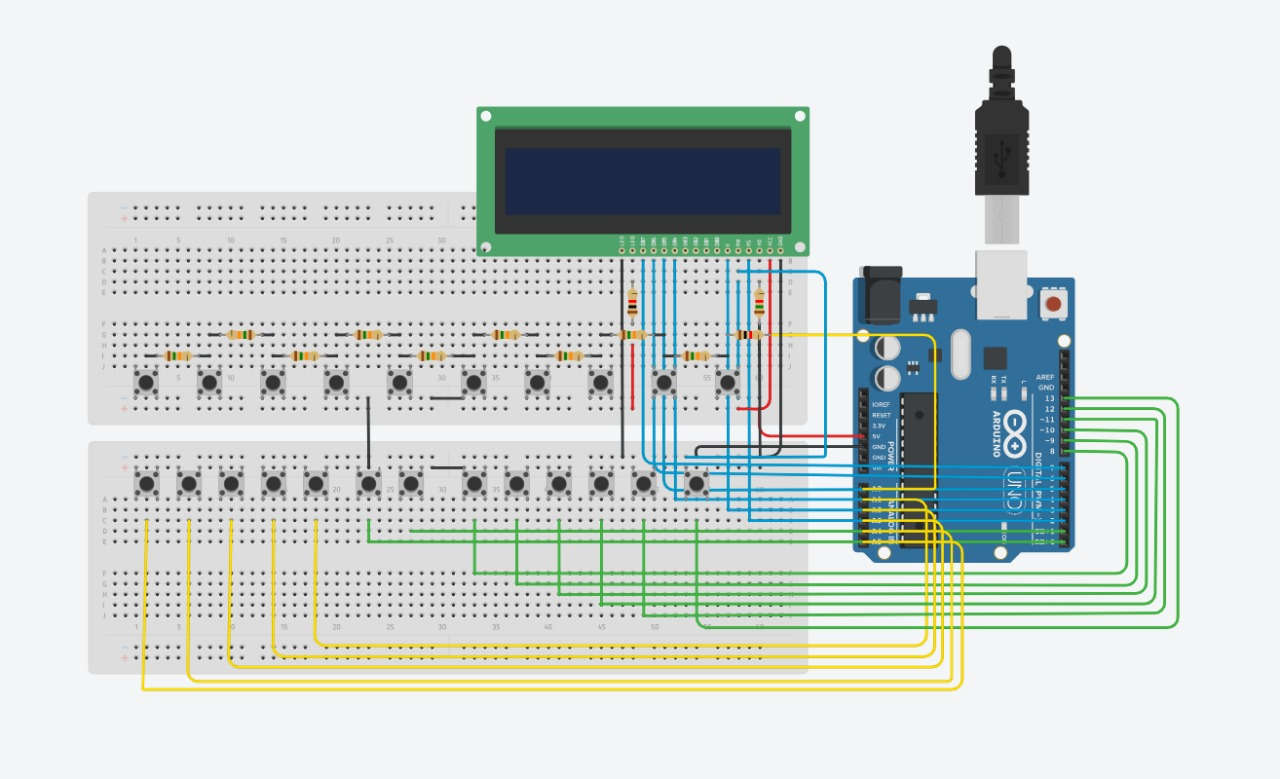
\includegraphics[width=\textwidth]{figs/image.jpeg}
        \label{fig:yourlabel}
\end{figure}
    \item Make the following connections to establish the required circuit:
        \begin{tabular}{|c|c|}  % Adjust columns as needed
        \hline
        \textbf{Pin(Arduino)} & \textbf{Connected To} \\  % Header row
        \hline
        2,3,4,5 & A,B,C,D of 7447 IC \\  
        \hline
        6,7,8,9,10,11 & COM of all the 6 displays  \\ 
        \hline
        5V, GND & $V_{cc}$ and GND of 7447 IC  \\  
        \hline
    \end{tabular}

     \newpage
\end{enumerate}
\textbf{Note:} Connections designed with the help of Akshara EE24BTECH11003,Teja vardhan EE24BTECH11034, Akshita EE24BTECH11054
\section{Software Implementation}
The Arduino code reads button inputs, processes mathematical operations, and displays the results on the LCD. The program initializes the LCD, manages user input, and executes the required functions using mathematical libraries. The key features of the software implementation include:
\begin{itemize}
\item Reading input from push buttons and mapping them to corresponding mathematical functions.
\item Displaying user inputs and results dynamically on the LCD.
\item Performing calculations using predefined mathematical functions in Arduino's library.
\item Handling errors such as invalid inputs or operations.
\item Implementing a real-time response mechanism to ensure smooth functionality.
\item Allowing easy modification of the code to add more functions in the future.
\end{itemize}
\section{Working Principle}
\begin{itemize}
\item The push buttons send signals to the Arduino, which interprets the input and processes the mathematical operations.
\item The LCD module displays the entered values and computed results.
\item The calculator follows a sequential operation mechanism where expressions are evaluated as they are entered.
\item Predefined mathematical functions such as trigonometric and logarithmic calculations are executed using Arduino libraries.
\item The system ensures accuracy by using floating-point arithmetic for precise calculations.
\item Error handling mechanisms prevent invalid inputs from disrupting calculations.
\end{itemize}
\section{Push Button Functions}
\begin{table}[H]
\centering
\caption{Push Button Designations}
\label{tab:functions}
\begin{tabular}{ccc}
\toprule
Button Number & Function \\
\midrule
1 - 10 & Digits 0 - 9 \\
11 & Clear \\
12 & $\ln{(x)}$ and $\log{(x)}$ \\
13 & Right Parenthesis \\
14 & $\sin{(x)}$, $\cos{(x)}$, and $\tan{(x)}$ \\
15 & $e$ and $\pi$ \\
16 & Backspace \\
17 & Decimal Point \\
18 & Equal To \\
19 & Left Parenthesis \\
20 & Division \\
21 & Multiplications \\
22 & Subtraction \\
23 & Addition \\
\bottomrule
\end{tabular}
\end{table}

\section{Results}
\begin{itemize}
\item The scientific calculator built using Arduino UNO performs mathematical operations accurately, displaying results clearly on the LCD.
\item The system successfully handles trigonometric, logarithmic, and arithmetic functions with reliable input from push buttons.
\item The calculator operates efficiently with minimal lag, and future improvements could include additional features like memory storage and touchscreen integration.
\end{itemize}
\section{Conclusion}
The scientific calculator using Arduino UNO successfully performs a range of mathematical operations, including arithmetic, trigonometric, and logarithmic functions. Future enhancements may include additional functions and an improved user interface. This project demonstrates the capability of Arduino for mathematical computing and provides a functional model for educational and practical applications. The successful implementation of this calculator showcases the feasibility of using microcontrollers for computational tasks in various fields.
\end{document}
